%\documentclass{article}
%\usepackage{tikz,pgfplots}
%\usepackage[pdftex,active,tightpage]{preview}
%\begin{document}
%\begin{preview}
%%%%%%%%%%%%%%%%%%%%%%%%%%%%%%%%%%
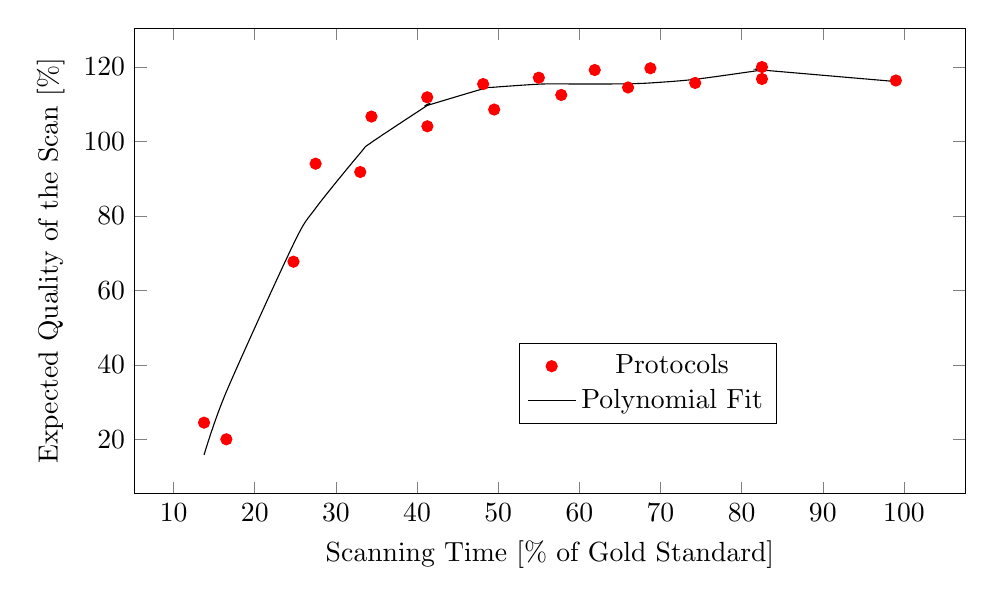
\begin{tikzpicture}

% defining custom colors
\definecolor{mycolor1}{rgb}{0,0.5,0}

\begin{axis}[%
	width=\linewidth,
	height=0.618\linewidth,
%	title={QualityPlot},%
	xlabel={Scanning Time [\%\ of Gold Standard]},%
	ylabel={Expected Quality of the Scan [\%]},%
	]

% Protocols
\addplot [ color = red, only marks, mark = *] 
coordinates{
 (13.7508,24.4684) (16.5009,20) (24.7703,67.7011) (27.5016,94.0267) (33.0019,91.7912) (34.3801,106.691) (41.2524,111.868) (41.2712,104.073) (48.1435,115.426) (49.5028,108.578) (55.0031,117.129) (57.7722,112.49) (61.8943,119.193) (66.0038,114.506) (68.7539,119.668) (74.2731,115.724) (82.5047,120) (82.5047,116.783) (99.0057,116.377)
};

% Line plot
\addplot [ smooth ] 
coordinates{
 (13.7508,15.7977) (16.5009,32.7737) (24.7703,72.4475) (27.5016,82.0774) (33.0019,96.8957) (34.3801,99.7454) (41.2524,109.67) (41.2712,109.689) (48.1435,114.145) (49.5028,114.578) (55.0031,115.394) (57.7722,115.456) (61.8943,115.425) (66.0038,115.504) (68.7539,115.723) (74.2731,116.7) (82.5047,119.19) (82.5047,119.19) (99.0057,116.093)
};

\pgfplotsset{every axis legend/.append style={
at={(0.618,0.2)},
anchor=base}}

\legend{Protocols,Polynomial Fit}%$p(x)=p_{1}x^{n}+p_{2}x^{n-1}+...+p_{n}x+p_{n+1}$}

\end{axis}

\end{tikzpicture}
%%%%%%%%%%%%%%%%%%%%%%%%%%%%%%%%%%
%\end{preview}
%\end{document}